%% LaTeX Beamer presentation template (requires beamer package)
%% see http://latex-beamer.sourceforge.net/
%% idea contributed by H. Turgut Uyar
%% template based on a template by Till Tantau
%% this template is still evolving - it might differ in future releases!

\documentclass[hyperref={pdfpagelabels=false}]{beamer}

\mode<presentation>

\usepackage{graphicx}
\usetheme{isu}
\usepackage{times}
\usepackage{amsmath,amsthm, amssymb, latexsym}
\boldmath
\usepackage[english]{babel}
\usepackage[utf8]{inputenc}
\usepackage{natbib}
\usepackage{listings}
\bibliographystyle{plainnat}

\DeclareGraphicsExtensions{.pdf,.jpg,.png}
\graphicspath{{figures/}}

\title[Proposal]{
    A Tale of Two Language Models:\linebreak
    Formally Validating Pig Compilation Algorithm
}
\author[Team Axum: David Johnston and Bijon Bose]{Team Axum: David Johnston and Bijon Bose}
\institute[ISU]{
    Department of Computer Science \linebreak
    Iowa State University\linebreak
    dwtj@iastate.edu\linebreak
    bkbose@iastate.edu
}

\date[COMS 641]{COMS 641: Data Intensive Languages and Systems - Design and Semantics}
%\date{Month X, 20XX}


% If you have a file called "university-logo-filename.xxx", where xxx
% is a graphic format that can be processed by latex or pdflatex,
% resp., then you can add a logo as follows:

%\pgfdeclareimage[height=0.25cm]{logo}{figures/logo}
%\logo{\pgfuseimage{logo}}


\begin{document}
  \begin{frame}[plain]
    \titlepage
  \end{frame}

  \section*{Overview}

\begin{frame}
\begin{itemize}
  \item The Problem
  \begin{itemize}
    \item Correctness of Pig programs depends upon correctness of compilation
          from Pig semantic model to the MapReduce semantic model.
  \end{itemize}

  \item Our Approach
  \begin{itemize}
    \item Coq: Formally model languages, semantics, compilation models; make
          correctness/equivalency proofs.
  \end{itemize}

  \item Evaluation
  \begin{itemize}
    \item Coq: Successfully write correctness proofs.
  \end{itemize}

  \item Benefits
  \begin{itemize}
    \item Formalization of both Pig and MapReduce semantic models can be reused.
    \item More advanced (i.e. optimizing) compilation algorithms can be modeled
          and validated.
  \end{itemize}

\end{itemize}
\end{frame}

  \section{The Problem}
%\begin{frame}
%  \frametitle{Course Rationale: Prevent This Class of Errors}
%  \begin{quote}
%      Language and framework-specific errors, i.e. errors that arise due to
%      incorrect understanding of the semantics of the language and/or framework
%      and its guarantees.
%  \end{quote}
%\end{frame}

\begin{frame}
  \frametitle{The Problem: Program Correctness Depends Upon Compilation
    Correctness}
  \begin{enumerate}
    \item Programs written in sequential, declarative style PigLatin are compiled to distributed Hadoop MapReduce jobs.
    \item A Pig program's correctness requires correct compilation.
    \item Correct compilation depends upon a non-trivial mapping from
      properties over Pig semantics to properties over MapReduce semantics through the transformation into Logical Plan and Physical Plan.
    \item Our goal is to prove the correctness of this compilation.
  \end{enumerate}
\end{frame}

  \section{Background}

\subsection{Pig-Latin Compilation}
\begin{frame}{Pig Latin Compilation}
\begin{itemize}
	\item Parser verifies the programs, performs type checking, schema inference
          and other tasks.
	\item It outputs a canonical logical plan with one-to-one mapping from each statement to 		  a node in logical plan.
	\item The logical plan is transformed to a physical plan where each logical operator is       		  simplified to corresponding physical operators.
	\item Pig assigns each physical operator to MapReduce stages with the goal of reducing   		  the number of reduce stages.
	
\end{itemize}
\end{frame}

%\subsection{MapReduce Execution Model}
%\begin{frame}{MapReduce Execution Model}
%\begin{itemize}
%	\item Map: Produces a stream of data items annotated with keys.
%	\item Local Sort: Orders the data at each machine by key.
%	\item Combiner: Performs partial aggregation on the locally ordered data.
%	\item Shuffle: Redistributes the data to achieve global ordering.
%	\item Merge/Combine: All data received at a particular machine is combined
%          into a single stream in merge stage.
%	\item Reduce: Finally the reduce stage processes the data associated with
%          each key and performs aggregation of the output results.
%\end{itemize}
%\end{frame}
%
%\begin{frame}{MapReduce Execution Model}
%\centerline{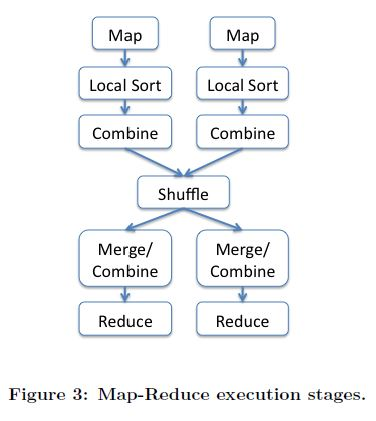
\includegraphics[scale=0.5]{Images/MapReduce_Execution.JPG}}
%\let\thefootnote\relax\footnotetext{\tiny\citet[VLDB][]{gates2009building}}
%\end{frame}

%\subsection{Pig Latin's Logical Plan}
%\begin{frame}{Logical Plan Structure}
%\begin{itemize}
%	\item A Pig Latin program is a sequence of steps, each of which carries out
%          a single transformation.
%	\item Each Pig Latin program is translated to a logical plan
%	\item Pig then translates the logical plan to a physical plan and embeds
%          each physical operator inside a MapReduce stage to arrive at the
%          MapReduce plan.
%\end{itemize}
%\end{frame}

\subsection{PigLatin - Logical Plan}
\begin{frame}{Logical Plan}
\centerline{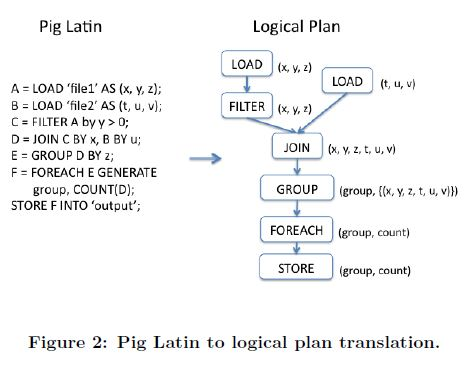
\includegraphics[scale=0.55]{Images/PigLatin.JPG}}
\let\thefootnote\relax\footnotetext{\tiny \citet[VLDB][]{gates2009building}}
\end{frame}

%\subsection{Generating MapReduce Jobs}
%\begin{frame}{Logical-MapReduce}
%\begin{itemize}
%	\item Pig translates the logical plan to a physical plan
%	\item Logical (CO)GROUP operator translates to - local rearrange, global
%          rearrange and package.
%	\item The JOIN is handled either with a COGROUP followed by a FOREACH or
%          fragment replicate join.
%	\item After the physical plan is generated Pig assigns physical operators to
%          Hadoop Stages
%\end{itemize}
%\end{frame}

\subsection{Logical Plan - Physical Plan}
\begin{frame}
\centerline{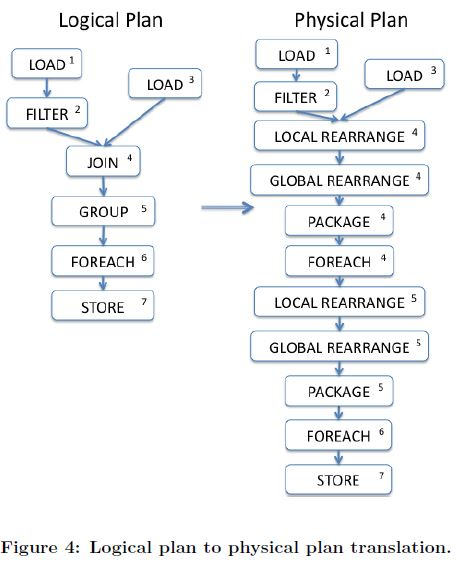
\includegraphics[scale=0.40]{Images/Logical_Physical.JPG} }
\let\thefootnote\relax\footnotetext{\tiny \citet[VLDB][]{gates2009building}}
\end{frame}

\subsection{Physical Plan - Map Reduce}
\begin{frame}
\centerline{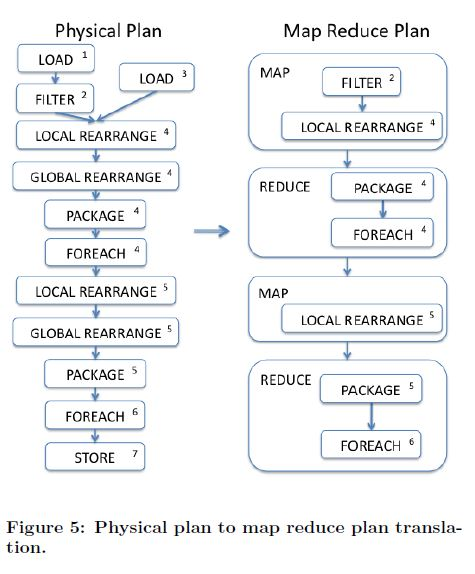
\includegraphics[scale=0.40]{Images/Physical_MapReduce.JPG}}
\let\thefootnote\relax\footnotetext{\tiny \citet[VLDB][]{gates2009building}}
\end{frame}

%\begin{frame}{Pig to MapReduce}
%\begin{itemize}
%	\item Pig compiles programs written in Pig Latin
%	\item Ultimately translates to Map-Reduce tasks
%	\item Pig also operates on local mode running on a single machine without
%          map-reduce
%	\item There lies an equivalence between PigLatin and MapReduce operational
%          semantics
%	\item The equivalence needs to be formalized and correctness needs to be
%          proved
%\end{itemize}
%\end{frame}


%\subsection{Three Main Papers}
%
%\begin{frame}{\citet[VLDB][]{gates2009building}}
%\emph{Building a HighLevel Dataflow System on top of MapReduce: The Pig
%Experience}:
%\begin{itemize}
%	\item This paper outlines the compilation phase of PigLatin programs and how
%          the logical plan of PigLatin is translated to actual Hadoop map-reduce
%          tasks.
%	\item But neither the semantics nor the compilation to map-reduce framework
%          have been formalized with proof of correctness.
%\end{itemize}
%\end{frame}
%
%\begin{frame}{\citet[SEFM]{ono2011using}}
%\emph{Using Coq in Specification and Program Extraction of Hadoop MapReduce
%Applications}
%\begin{itemize}
%    \item Constructed formal model of MapReduce computation in Coq where:
%    \begin{itemize}
%        \item Model user-defined map/reduce as Coq functions
%        \item Application specifications are defined as invariants
%    \end{itemize}
%	\item Constructed formal model of the (previously informally specified)
%          Hadoop libraries
%	\item Using these, they prove the correctness of some example MapReduce
%          applications.
%    \item Future Work: Investigate a more MapReduce applications
%\end{itemize}
%\end{frame}
%
%\begin{frame}{\citet[Journal of Automated Reasoning][]{leroy2009formally}}
%\emph{A formally verified compiler back-end}
%\begin{itemize}
%	\item Compcert: Formally verified compiler from Cminor to PPC assembly.
%    \item Programmed and proven sound using Coq.
%    \item Lots of background on compiler verification.
%\end{itemize}
%\end{frame}

  \section{Our Approach}

\subsection{Pig Latin Features}
\begin{frame}{Features}
\begin{itemize}
	\item DataFlow Language:
	\begin{itemize}
		\item Programmer defines a sequence of statements where each carries out a single 					  data transformation. The output relation of each statement is stored in an  					  identifier to be used later in the program.
	\end{itemize}
	\item User Defined Functions:
	\begin{itemize}
		\item User defined functions provide the flexibility to perform specialized data 				 	  processing tasks.
	\end{itemize}
	\item Abstract Parallelism:
	\begin{itemize}
		\item Pig Latin programs are represented a sequential way to define the query 					      statements abstracting away the underlying parallelism performed through the 					  map-reduce tasks.
	\end{itemize}
\end{itemize}
\end{frame}

\subsection{Formalism}
\begin{frame}{Four Stages of Pig Programs}
\begin{itemize}
	\item A Pig Latin program passes through four stages of compilation:
	\begin{itemize}
		\item Pig Latin Program
		\item Logical Plan
		\item Physical Plan
		\item Map Reduce Phase
	\end{itemize}
	\item The logical plan is an one-to-one mapping from Pig Latin Program and the in Map-				  Reduces phase is executed by assigning physical operators to corresponding map-				  reduce jobs. So we've started our formalism by defining the calculus for Logical 				  plan and Map-Reduce in terms of Pig Latin programs.
\end{itemize}
\end{frame}

\subsection{Formalism for Logical Plan}

\begin{frame}{Conventions}
\centering
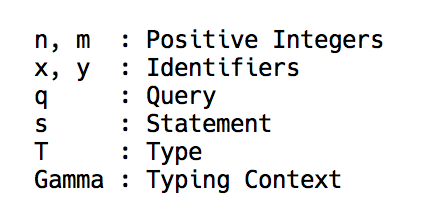
\includegraphics[scale=0.80]{conventions}
\end{frame}

\begin{frame}{Grammar: Queries}
\centering
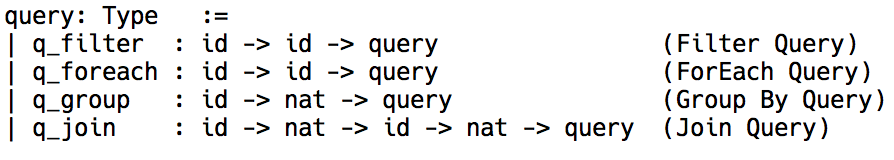
\includegraphics[scale=0.60]{query}
\end{frame}

\begin{frame}{Grammar: Statements}
\centering
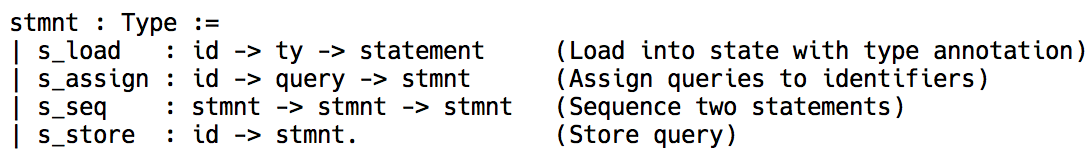
\includegraphics[scale=0.60]{stmnt}
\end{frame}

\begin{frame}{Types}
\centering
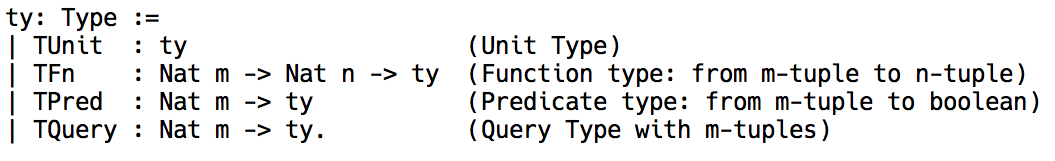
\includegraphics[scale=0.60]{ty}
\end{frame}

\begin{frame}{Typing Rules: Queries}
\centering
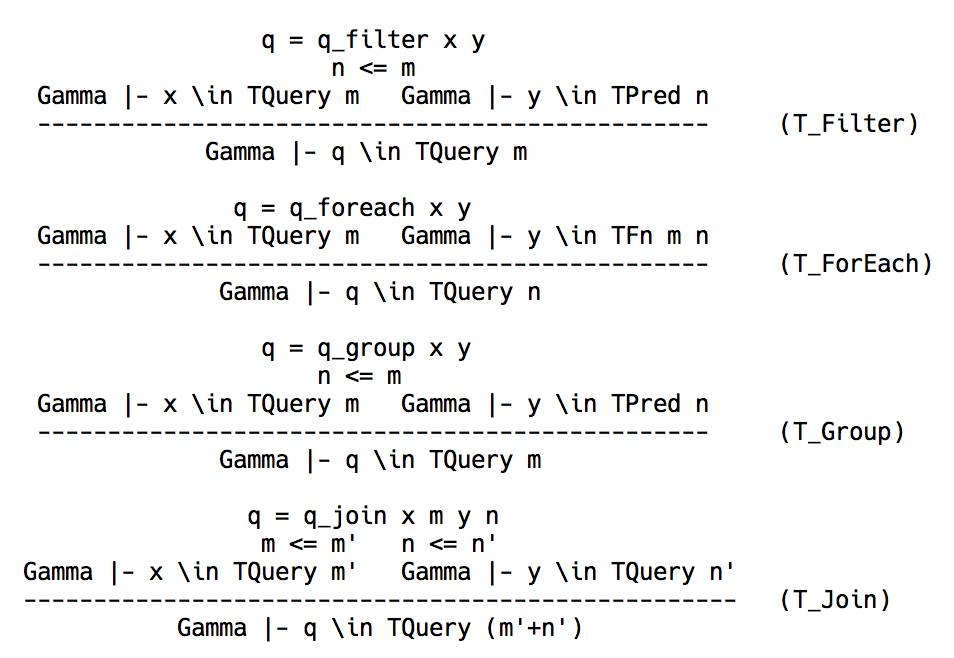
\includegraphics[scale=0.50]{T_Queries}
\end{frame}

\begin{frame}{Typing Rules: Statements}
\centering
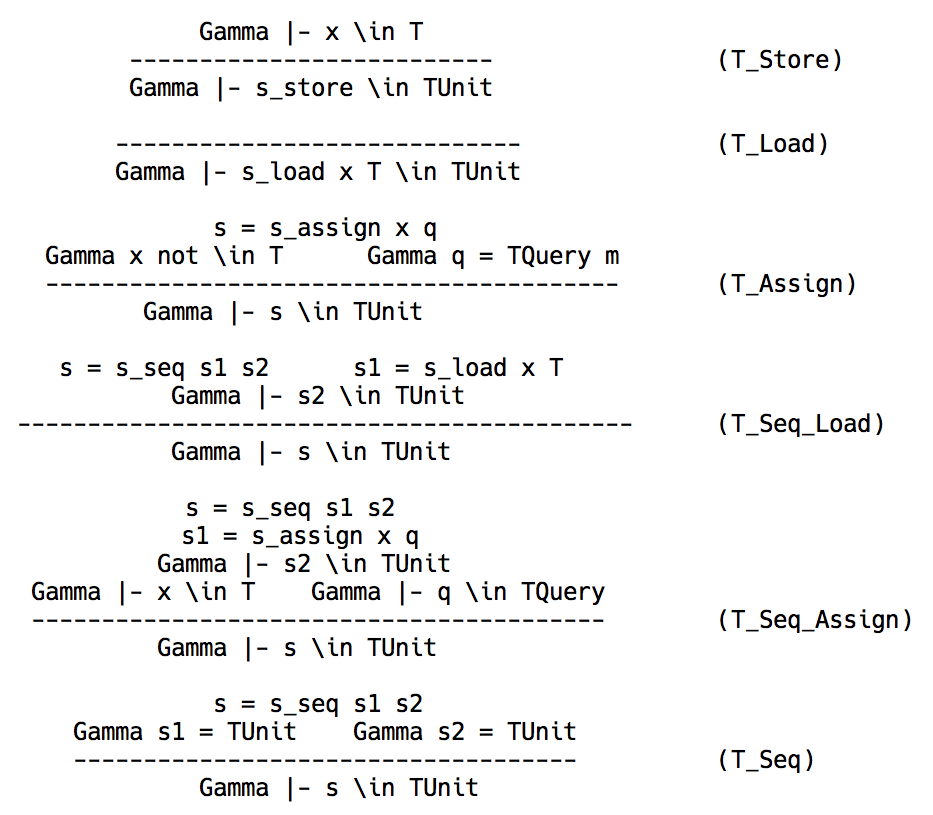
\includegraphics[scale=0.40]{T_Statements}
\end{frame}

  \section{Challenges}

\begin{frame}{Challenges}
To challenges in the formalization for Pig Latin are -
\begin{itemize}
	\item To identify and differentiate between the different phases of PigLatin
	\item Develop core semantics for each phases while maintaining the core features of Pig Latin
	\item How to represent the equivalence between different phases
\end{itemize}
\end{frame}

  %\section*{Related Work}

\subsection{Pig Latin}
\begin{frame}
  \begin{itemize}
    \item \citet[SIGMOD][]{olston2008pig} \\
          \emph{Pig-Latin: A not-so-foreign language for data processing}
    \item \citet[VLDB][]{gates2009building} \\
          \emph{Building a high-level dataflow system on top of Map-Reduce: the
          Pig experience}
    \item \citet[TASS][]{zhang2013performance} \\
          \emph{Performance Modeling and Optimization of Deadline-Driven Pig
          Programs}
  \end{itemize}
\end{frame}

\subsection{MapReduce Model}
\begin{frame}
  \begin{itemize}
    \item \citet[CACM][]{dean2004mapreduce} \\
          \emph{MapReduce: Simplified Data Processing on Large Clusters}
    \item \citet[SIGMOD][]{yang2007map} \\
          \emph{Map-reduce-merge: Simplified relational data processing on large
          clusters}
    \item \citet[ICSE][]{xiao2014nondeterminism} \\
          \emph{Nondeterminism in mapreduce considered harmful? ...}
    \item \citet[ASPLOS][]{leesatapornwongsa2016taxdc} \\
          \emph{TaxDC: A Taxonomy of Non-Deterministic Concurrency Bugs in
          Datacenter Distributed Systems}
  \end{itemize}
\end{frame}

\subsection{Formalisms and Correct Usage of MapReduce}
\begin{frame}[allowframebreaks]
  \begin{itemize}
    \item \citet[Science of Computer Programming][]{lammel2008google} \\
          \emph{Google's MapReduce programming model--Revisited}
    \item \citet[ABZ][]{pereverzeva2014formal} \\
          \emph{Formal Derivation of Distributed MapReduce}
    \item \citet[TACAS][]{chen2015commutativity} \\
          \emph{Commutativity of Reducers}
    \item \citet[Concurrency and Computation][]{dorre2015modeling} \\
          \emph{Modeling and optimizing MapReduce programs}
    %\item \citet[ECBS][]{yang2010formalizing} \\
    %      \emph{Formalizing MapReduce with CSP}
    \item \citet[SEFM][]{ono2011using} \\
          \emph{Using Coq in Specification and Program Extraction of Hadoop
          MapReduce Applications}
  \end{itemize}
\end{frame}

  \section*{}

%\textsc{\textsc{\textsc{\begin{frame}{Future Work}
  %\begin{itemize}
    %\item % TODO Talk about future work/limitations here
  %\end{itemize}
%\end{frame}


%\begin{frame}{Conclusion}
% TODO copy/paste overview here (from intro.tex)
%\end{frame}}


\begin{frame}
\begin{beamercolorbox}[center]{white}
  {\Large Questions?}

  \vspace{2em}\hfill

  \url{https://github.com/isu-cs641s16-axum}
\end{beamercolorbox}
\end{frame}


  \begin{frame}[allowframebreaks]
    \bibliography{refs}{}
  \end{frame}
  \appendix

% make sure you have a blank slide in case you accidentally go past your conclusion
\begin{frame}[plain]
\end{frame}


% these slides are to help answer potential questions and generally arent shown
% unless needed or there is extra time
\begin{frame}[plain]{Hidden Slide 1}
\end{frame}

\begin{frame}[plain]{Hidden Slide 2}
\end{frame}

\end{document}
